\input{Preamble.tex}

\usepackage{subfigure}

\begin{document}

%%%%%%%%%%%%%%%%%%%%%%%%%%%%%%%%%%%%%%%%%%%%%%%%%%%%%%%%%%%%%%%%%%%%%%%%% 
%								CARATULA								%
%%%%%%%%%%%%%%%%%%%%%%%%%%%%%%%%%%%%%%%%%%%%%%%%%%%%%%%%%%%%%%%%%%%%%%%%% 

\begin{titlepage}

\newcommand{\HRule}{\rule{\linewidth}{0.5mm}}
\center
\mbox{\textsc{\large \bfseries {INSTITUTO TECNOLÓGICO DE BUENOS AIRES}}}\\[1cm]
\textsc{\Large 22.42 Laboratorio de Electrónica}\\[0.5cm]


\HRule \\[0.6cm]
{ \Huge \bfseries Trabajo Práctico N$^{\circ}$4}\\[0.4cm] 
\HRule \\[1.5cm]


{\large

\emph{Grupo 3}\\
\vspace{3px}

\begin{tabular}{lr} 	
\textsc{Bertachini}, Germán  & 58750 \\ 	
\textsc{Lambertucci}, Guido Enrique  & 58009 \\
\textsc{Londero Bonaparte}, Tomás Guillermo  & 58150 \\
\textsc{Mechoulam}, Alan  &  58438\\
\textsc{Scapolla}, Franco & 58465
\end{tabular}

\vspace{20px}

\emph{Profesores}\\
\vspace{3px}
\textsc{Cossutta}, Pablo Martín\\
\textsc{Weill}, María\\
\textsc{Salvati}, Matías\\	
\vspace{100px}

\begin{tabular}{ll}

Presentado: & 15/10/19\\

\end{tabular}

}

\vfill

\end{titlepage}



%%%%%%%%%%%%%%%%%%%%%%%%%%%%%%%%%%%%%%%%%%%%%%%%%%%%%%%%%%%%%%%%%%%%%%%%% 
%								INFORME									%
%%%%%%%%%%%%%%%%%%%%%%%%%%%%%%%%%%%%%%%%%%%%%%%%%%%%%%%%%%%%%%%%%%%%%%%%%

%%%%%TABLE OF CONTENTS
\tableofcontents
\newpage


\section{Introducción}
En el presente trabajo de laboratorio se estudian filtros RLC de segundo orden, haciendo uso del osciloscopio, el generador de funciones y el analizador de impedancias. También, se realiza un programa para automatizar las mediciones del osciloscopio; dicho programa será de gran utilidad en trabajos prácticos futuros.

\section*{Caracterización de componentes pasivos}

\subsection*{Inductancia}
A continuación, se realizará un estudio acerca del comportamiento de una bobina, observando como varían sus magnitudes según la frecuencia y analizando sus circuitos equivalentes.\par En un sistema simplificado, la bobina sólo tiene un componente inductivo, sin embargo, dicho planteo dista en gran medida de la realidad donde, debido en gran medida a su fabricación, las inductancias tendrán tanto componentes resistivos como capacitivos. \par Las características previamente mencionadas nos llevarán a plantear distintos circuitos equivalentes. Se analizará cual de ellos refleja en mejor medida la práctica experimental realizada.

Para comenzar, se realiza el estudio de las magnitudes propias del inductor en función de la frecuencia. \par Las frecuencias utilizadas fueron detectadas ya que eran las que permitían ver con claridad como variaba la fase. Las mediciones se tomaron en el modo serie del analizador de impedancias, las mismas se pueden apreciar en la tabla (\ref{table:Rta_en_frecuencia_inductor}).

La inductancia provista por la cátedra tiene un valor de $500\mu H$.

Se plantea el siguiente circuito equivalente:

%circuito equivalente Inductancia
\begin{figure}[H]
\centering
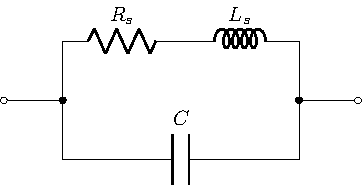
\includegraphics[width=6cm,height=4cm]{Ejercicio_1(Germo)/Circuitos/circuito_equivalente_inductancia.pdf}
\label{fig:circuito_equivalente_inductancia}
\end{figure}
%~circuito equivalente Inductancia

Al ser las bobinas un conjunto de espiras enrolladas una gran cantidad de vueltas, el componente resistivo de la inductancia se debe a la resistencia eléctrica del material utilizado en su fabricación. También, se podría considerar la resistencia propia de los terminales.
Por otro lado, debido a que consctructivamente cada una de las vueltas de la bobina están aisladas eléctricamente entre si debido al barniz que recubre el material y a la pequeña diferencia de tensión, se puede apreciar el comportamiento de un capacitor entre vuelta y vuelta del cable.


%% Tabla inductor
 \begin{center}
     \begin{table}[H]
     \centering
     \renewcommand{\arraystretch}{1.1}
     \scalebox{0.8}{
         \begin{tabular}{ c c c c c c }
            \hline 
             $\bm{f_S[Hz]}$ &  $\bm{L_S[mH]}$ & $\bm{Q}$& $\bm{R_S[\Omega]}$ & $\bm{|Z|[\Omega]}$ & $\bm{\theta}[^\circ]$ \\
             \hline
                10		& 0.490        & 0.0    & 0.91 		& 0.96  & 18.7   \\
				100 	& 0.480       & 3.0   	 & 0.10  	& 0.32  & 72.0     \\
				1K    & 0.480         & 16.6	& 0.18 		& 3.02  & 86.0     \\
				5K    & 0.485        & 25.8 	& 0.59		 & 15.23 & 87.8   \\
				10K   & 0.482        & 26.0     & 1.16 		& 30.32 & 87.8   \\
				20K   & 0.478       & 23.8 		& 2.52 		& 60.11 & 87.6   \\
				30K   & 0.474       & 22.1 		& 4.04 		& 89.35 & 87.4  \\
				50K   & 0.467        & 19.5		 & 7.50 		 & 146.70 & 87.1  \\
				75K   & 0.462       & 16.7 		& 13.00   	& 217.80 & 86.6  \\
				100K  & 0.459       & 14.4 		& 20.00  	 & 289.20 & 86.0   \\
				200K  & 0.466       & 8.6  		& 67.70 	& 589.50 & 83.4    \\
				400K  & 0.529        & 4.1 		 & 322 		 & 1368  & 76.4   \\
				450K  & 0.556        & 3.5 		 & 450  	& 1635  & 74.1   \\
				500K  & 0.589        & 2.9 		 & 632 		 & 1954  & 71.2  \\
				550K  & 0.627        & 2.4  	& 893  		& 2344  & 67.6    \\
				600K  & 0.669        & 2.0    & 1281 		& 2829  & 63.1   \\
				650K  & 0.708        & 1.5 		 & 1868 	& 3442  & 57.1    \\
				700K  & 0.724       & 1.2  		& 2763 		& 4217  & 49.1    \\
				725K  & 0.711        & 1.0  	  & 3356	 & 4664  & 44.0    \\
				750K  & 0.671       & 0.8 		 & 4060 	& 5147  & 38.0    \\
				775K  & 0.595       & 0.6 		 & 4831 	& 5633  & 31.0       \\
				800K  & 0.472       & 0.4 		 & 5608 	& 6089  & 22.9       \\
				825K  & 0.301       & 0.2  		& 6264 		& 6456  & 14.0       \\
				850K  & 0.094        & 0.1  	& 6653		& 6672  & 4.4        \\
				855K  & 0.053       & 0.0  		  & 6692	 & 6698  & 2.5        \\
				862K5 & -0.100         & 0.0    & 6715 		& 6715  & -0.5       \\
				870K  & -0.719       & 0.1 		 & 6706 	& 6718  & -3.4        \\
				875K  & -0.111      & 0.1  		& 6677 		& 6705  & -5.3       \\
				900K  & -0.290      & 0.3  		& 6356 		& 6563  & -14.4      \\
				925K  & -0.421      & 0.4 		 & 5787		 & 6282  & -22.9      \\
				950K  & -0.500         & 0.6  	& 5114 		& 5921  & -30.3       \\
				1M    & -0.549      & 0.9  		& 3820		 & 5146  & -42.1      \\
				1M1  & -0.470      & 1.5  		& 2132		 & 3884  & -56.7      \\
				1M2  & -0.368      & 2.1  		& 1306 		& 3068  & -64.8      \\
				1M3   & -0.291      & 2.7  		& 874  		& 2531  & -69.8      \\
				1M4  & -0.235      & 3.3 		 & 626  	& 2159  & -73.2     \\
				2M    & -0.093      & 6.7 		 & 175 		 & 1179  & -81.5       \\
				4M    & -19.79$*10^-3$  & 16.8 		& 29.6		 & 498.4 & -86.6     \\
				10M   & -2.893$*10^-3$ & 27.3 		& 6.7  		& 181.9 & -87.9     \\
            \hline 
        \end{tabular}
        }
        \caption{Magnitudes del inductor en función de la frecuencia}
        \label{table:Rta_en_frecuencia_inductor}
    \end{table}
\end{center}
%%~Tabla inductor

\subsection{Capacitor}
Se procederá a realizar el mismo análisis planteado anteriormente para una inductancia pero, para este caso con un capacitor, analizando como varían sus magnitudes según la frecuencia a la que trabaja y el estudio de sus circuitos equivalentes.

Para comenzar, se realiza el estudio de las magnitudes propias del capacitor en función de la frecuencia. \par Las frecuencias utilizadas fueron detectadas ya que eran las que permitían ver con claridad como variaba la fase. Las mediciones se tomaron en el modo paralelo del analizador de impedancias por lo que se medirán conductancias. Las mismas se pueden apreciar en la tabla (\ref{table:Rta_en_frecuencia_capacitor}).

El capacitor utilizado fue el provisto por la cátedra para el Trabajo Práctico N°1 de $2.2nF$

Se plantea el siguiente circuito equivalente:

%circuito equivalente capacitor
\begin{figure}[H]
\centering
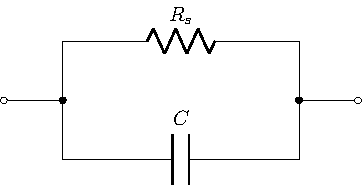
\includegraphics[width=6cm,height=4cm]{Ejercicio_1(Germo)/Circuitos/circuito_equivalente_capacitor.pdf}
\label{fig:circuito_equivalente_capacitor}
\end{figure}
%~circuito equivalente capacitor


La resistencia observada se debe a la resistencia eléctrica del material del componente(film).También, se podría considerar la resistencia propia de los terminales. \par
Por otro lado, se podría considerar una inductancia en el modelo equivalente pero debido al método de fabriacación y por las frecuencias con las que se puede trabajar en el laboratorio no se pudo hallar una frecuencia donde se apreciará un comportamiento de tipo inductivo. El máximo cambio de fase obtenido fue de aproximadamente $4^\circ$ a $13 MHz$.


%% Tabla capacitor
 \begin{center}
 
     \begin{table}[H]
     \centering
     \renewcommand{\arraystretch}{1.1}
     \scalebox{0.8}{
         \begin{tabular}{ c c c c c c c c }
            \hline 
             $\bm{f_P[Hz]}$ &  $\bm{C_P[nF]}$ & $\bm{D}$& $\bm{R_P[S]}$ & $\bm{|Z|[S]}$ & $\bm{\theta}[^\circ]$ \\

             \hline
             10   & 2.2  & 0.000 & 0.00       & 0.14$\mu$   & 89.9  \\
			100  & 2.27 & 0.010 & 0.00       & 1.43$\mu$   & 89.90 \\
			1K   & 2.26 & 0.004 & 0.05$\mu$   & 14.22$\mu$  & 89.80 \\
			5K   & 2.25 & 0.007 & 0.49$\mu$   & 70.73$\mu$  & 89.60 \\
			10K  & 2.24 & 0.007 & 1$\mu$ & 0.14$m$ & 89.56 \\
			20K  & 2.23 & 0.010 & 3$\mu$ & 0.28$m$ & 89.42 \\
			30K  & 2.23 & 0.011 & 5$\mu$  & 0.42$m$    & 89.35 \\
			50K  & 2.22 & 0.013 & 9$\mu$  & 0.70$m$  & 89.28 \\
			75K  & 2.21 & 0.014 & 14$\mu$  & 1.04$m$   & 89.22 \\
			100K & 2.21 & 0.014 & 19$\mu$   & 1.38$m$   & 89.21 \\
			200K & 2.19 & 0.015 & 42$\mu$   & 2.75$m$  & 89.30 \\
			400K & 2.18 & 0.016 & 88$\mu$   & 5.47$m$   & 89.08 \\
			450K & 2.17 & 0.016 & 100$\mu$    & 6.15$m$  & 89.07 \\
			500K & 2.17 & 0.016 & 111$\mu$   & 6.82$m$  & 89.06 \\
			550K & 2.12 & 0.017 & 124$\mu$   & 7.40$m$    & 89.06 \\
			650K & 2.17 & 0.017 & 149$\mu$   & 8.84$m$   & 89.04 \\
			750K & 2.16 & 0.017 & 173$\mu$   & 10.20$m$   & 89.03 \\
			800K & 2.16 & 0.017 & 186$\mu$   & 10.87$m$  & 89.02 \\
			900K & 2.16 & 0.017 & 210$\mu$    & 12.22$m$  & 89.01 \\
			1M   & 2.16 & 0.018 & 240$\mu$    & 13.57$m$  & 89.00 \\
			1M2  & 2.16 & 0.018 & 290$\mu$    & 16.27$m$  & 88.97 \\
			2M   & 2.16 & 0.019 & 520$\mu$    & 27.12$m$ & 88.90 \\
			4M   & 2.2  & 0.023 & 1.270$m$   & 55.38$m$  & 88.68 \\
			7M   & 2.3  & 0.032 & 3.200$m$    & 101.05$m$ & 88.16 \\
			9M   & 2.43 & 0.039 & 0.005   & 0.13  & 87.70 \\
			11M  & 2.63 & 0.050 & 0.009   & 0.18   & 87.10 \\
			12M  & 2.76 & 0.057 & 0.012   & 0.21   & 86.70 \\
			13M  & 2.91 & 0.065 & 0.015   & 0.24   & 86.30 \\
            \hline 
        \end{tabular}
        }
        \caption{Magnitudes del capacitor en función de la frecuencia}
        \label{table:Rta_en_frecuencia_capacitor}
    \end{table}
\end{center}
%%~Tabla capacitor


\section{Filtro pasabajos}

En esta sección se analizó la respuesta al escalón del circuito mostrado en la Figura (\ref{fig:rlc}). Sabiendo que $L = 500 \ \mu H$, $C = 33 \ nF$ y $\xi = 0.33$, se determinó que $R = 81.24 \ \Omega$. Además, se calculó la frecuencia de resonancia de este circuito, siendo esta $f_0 = 39.2 \ kHz$. Para determinar R se analizó primero la transferencia. Tenemos que la función transferencia del circuito es:

\begin{equation}
	H(s) = \frac{1}{LC s^2 + RC s + 1}
	\label{equ:hrlc}
\end{equation}

Sabiendo que $w_0=\frac{1}{\sqrt{LC}}$ y escribiendo el denominador de $H(s)$ la forma $1+2\xi\frac{s}{w_0}+(\frac{s}{w_0})^2$ obtenemos \begin{equation}
    H(s)=\frac{1}{1+RC\frac{1}{\sqrt{LC}}\frac{s}{\frac{1}{\sqrt{LC}}}+(\frac{s}{\frac{1}{\sqrt{LC}}})^2}=\frac{1}{1+R\sqrt{\frac{C}{L}}\frac{s}{w_0}+(\frac{s}{w_0})^2}
\end{equation}
Por lo tanto, se tiene que $2\xi=R\sqrt{\frac{C}{L}}$, de donde como $\xi=0,33$, $L=500\mu H$ y $C=33nF$, se encuentra $R=81,24\Omega$


\begin{figure}[H]
\begin{center}
\begin{circuitikz}
	\node [buffer](buff){};
	\draw (buff.out) to[short] ++(0.25,0) to[L, l = $L$] ++(2,0) to[R, l = $R$] ++(2.5,0) node[](Vcpos){};
	\draw (Vcpos) to[C, l_= $C$, v^= $V_C$] ++(0,-2) node[](Vcneg){};
	\draw (buff.in) to[short] ++(-0.5,0) to[sV, v_=$V_i$] ++(0,-2) to[short] node[ground]{} (Vcneg);
\end{circuitikz}
\caption{Primera etapa del circuito.}
	\label{fig:rlc}
\end{center}
\end{figure}

Luego se procedió a analizar distintos valores de importancia del circuito, como lo son la frecuencia de oscilación del transitorio, el tiempo de establecimiento del $5 \ \%$ y el sobre pico. Para ello se analiza nuevamente la transferencia del circuito hallada en (\ref{equ:hrlc})

\begin{equation*}
	H(S) = \frac{1}{LC S^2 + RC S + 1}
	\label{equ:hrlc}
\end{equation*}

Es así que, sabiendo que la transformada de Laplace del escalón es $\frac{1}{S}$, y la salida del sistema es $Y(S) = X(S) \cdot H(S)$, se obtuvo la respuesta al escalón de este:

\begin{equation} \hspace*{-1cm}
	V_{C}(t) = 1 - e^{-t \frac{R}{2L}} \cdot \left[\frac{1}{2 \sqrt{4LC - {RC}^2}} \cdot sen \left( \frac{\sqrt{4LC - {RC}^2}}{2LC} \cdot t \right) + cos \left( \frac{\sqrt{4LC - {RC}^2}}{2LC} \cdot t - \pi \right) \right]
	\label{equ:vc}
\end{equation} 

Además, se sabe que la frecuencia de oscilación del transitorio se puede calcular como

\begin{equation}
	f_t = f_0 \cdot \sqrt{|\xi^2 - 1|} = 37 \ kHz
	\label{equ:fres}
\end{equation}

Por otro lado, el sobre pico se calcula como 

\begin{equation}
    M_p=e^{\frac{-\xi\pi}{\sqrt{1-\xi^2}}}=333mV
    \label{equ:mp}
\end{equation}

Finalmente, el tiempo de establecimiento del $5\%$ puede calcularse de (\ref{equ:vc}) tomando la envolvente de la respuesta al escalón y resolviendo:

\begin{equation}
	e^{-t\frac{R}{2L}} = 0.05
\end{equation}

\begin{equation}
	t=36.87\mu s
\end{equation}

Considerando los valores comerciales, y sabiendo que se disponía de una bobina de una inductancia de $500 \ \mu H$, se utilizaron una resistencia de $82 \ \Omega$ y un capacitor de $33 \ nF$. Es así que se preparó el circuito en un protoboard y se procedió a realizar las mediciones pertinentes y así compararlas con los cálculos teóricos. Este circuito fue excitado con una señal cuadrada, la cual posee una frecuencia de $3.92 \ kHz$, un décimo de la frecuencia de resonancia, y una amplitud tal que la tensión de salida máxima sea de $1 \ V_{pp}$. Es así que se observó la respuesta al escalón del sistema, al inicio de cada cuadrada.

\begin{figure}[H]
	\centering
	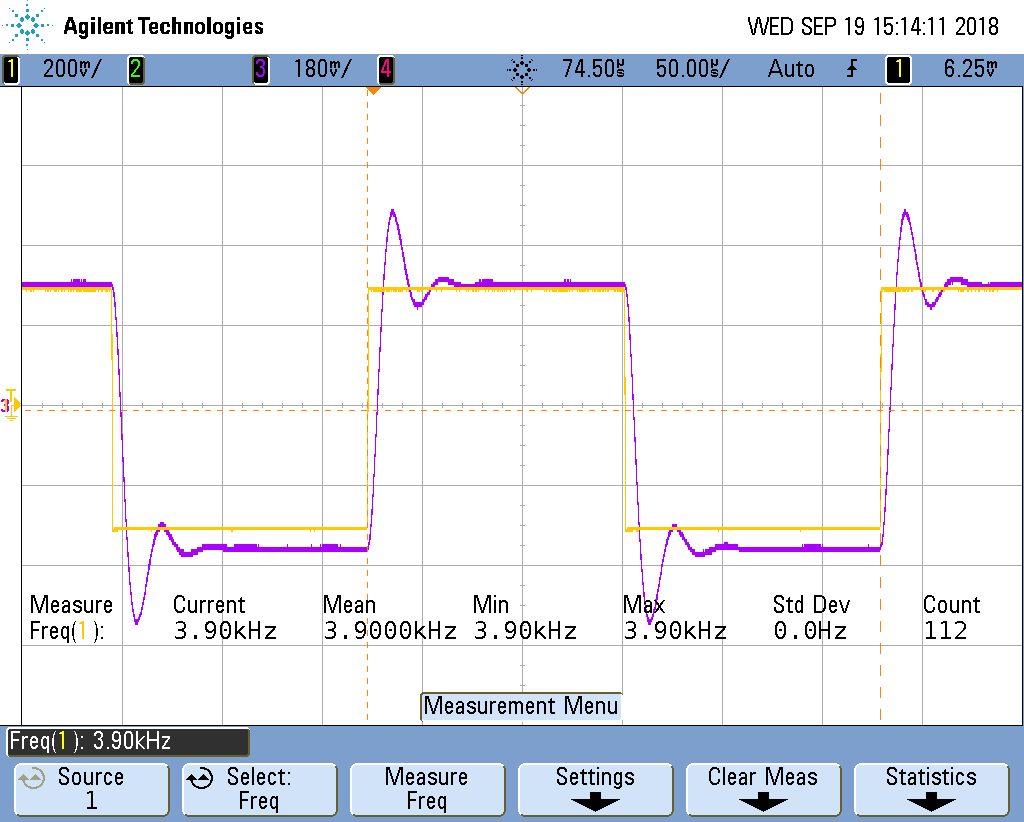
\includegraphics[width=0.9\textwidth, trim = {0 3.4cm 0.4cm 2cm},clip]{Ejercicio2/Mediciones/A/waveform2.png}
\caption{Respuesta al escalón del circuito.}
	\label{fig:rtaescalon}
\end{figure}

De esta forma, se midió una frecuencia de oscilación de $41 \ KHz $, un sobre pico de $245 \ mV$ y un tiempo de establecimiento del 5\% de $33.6 \ \mu s$. Las discrepancias entre los valores teóricos y los medidos pueden deberse a varios factores. Uno de los más importantes es la capacitancia que añaden las puntas al circuito.

Se puede observar como, inyectada una señal cuadrada al circuito, existe un pequeño tiempo de establecimiento oscilatorio. A continuación, se realizó un barrido desde la frecuencia utilizada anterior mente hasta una frecuencia 20 mayor. A continuación se muestran los resultados:

\begin{figure}[H]
\centering
\begin{subfigure}
  \centering
  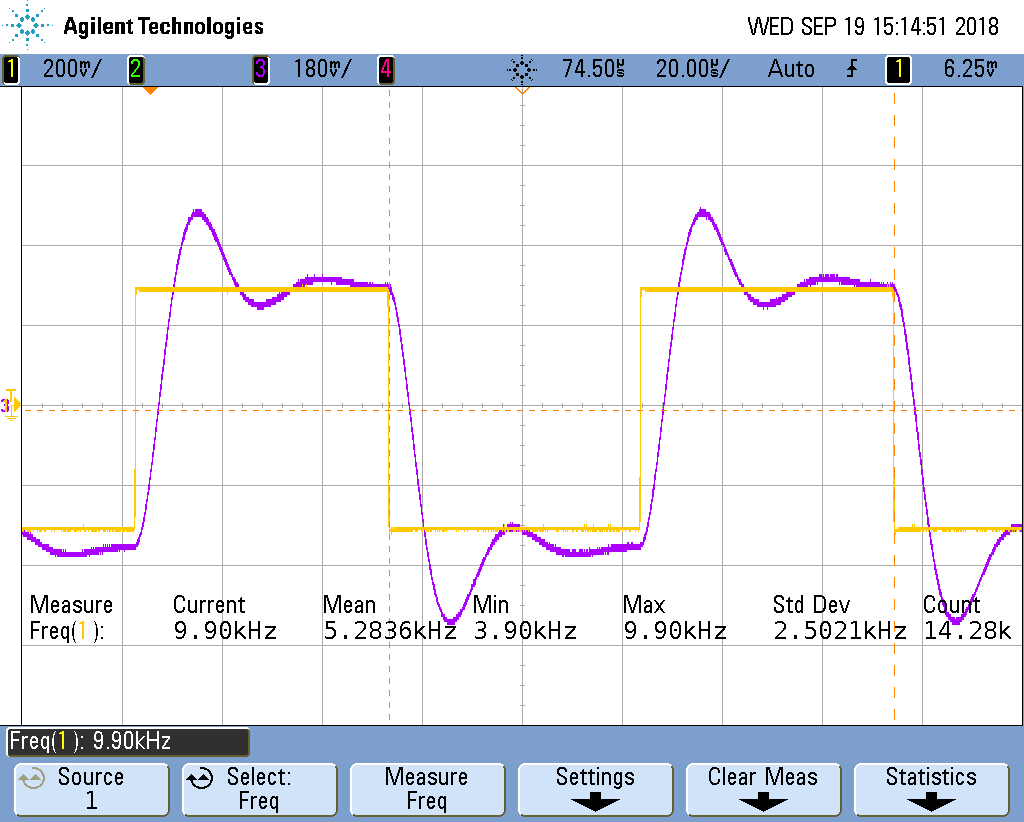
\includegraphics[width=.8\textwidth]{Ejercicio2/Mediciones/A/waveform3.png}  
\end{subfigure}
\begin{subfigure}
  \centering
  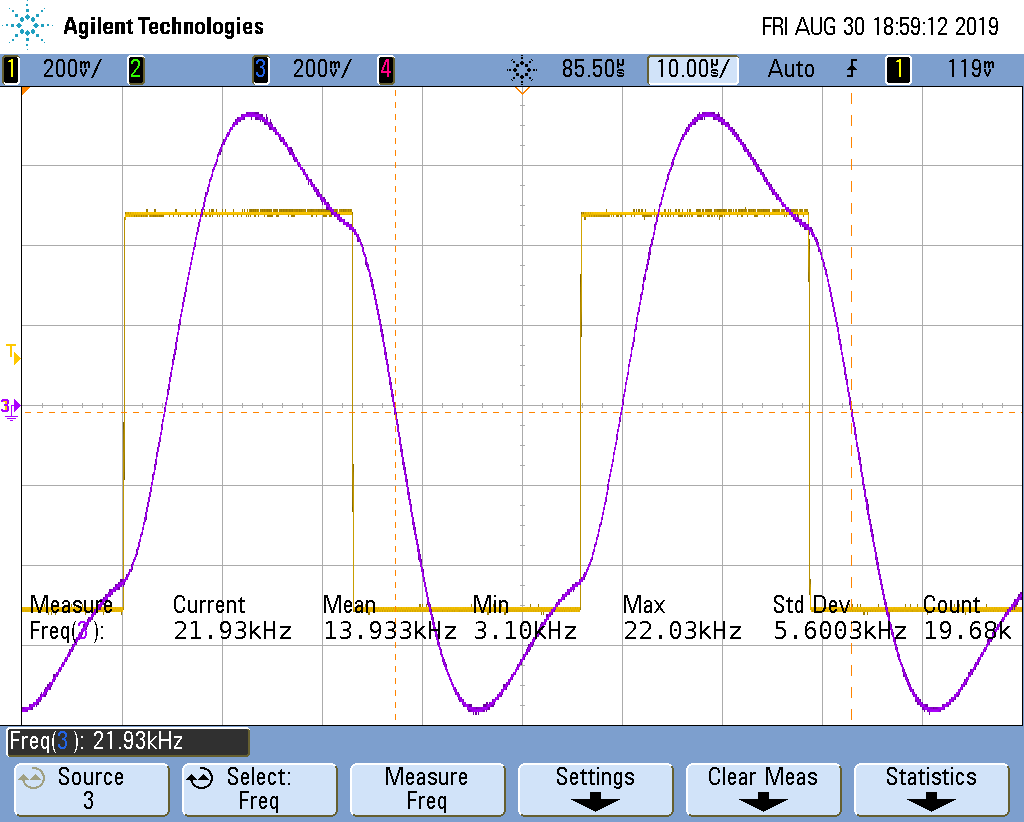
\includegraphics[width=.8\textwidth]{Ejercicio2/Mediciones/A/waveform4.png}  
\end{subfigure}
\begin{subfigure}
  \centering
  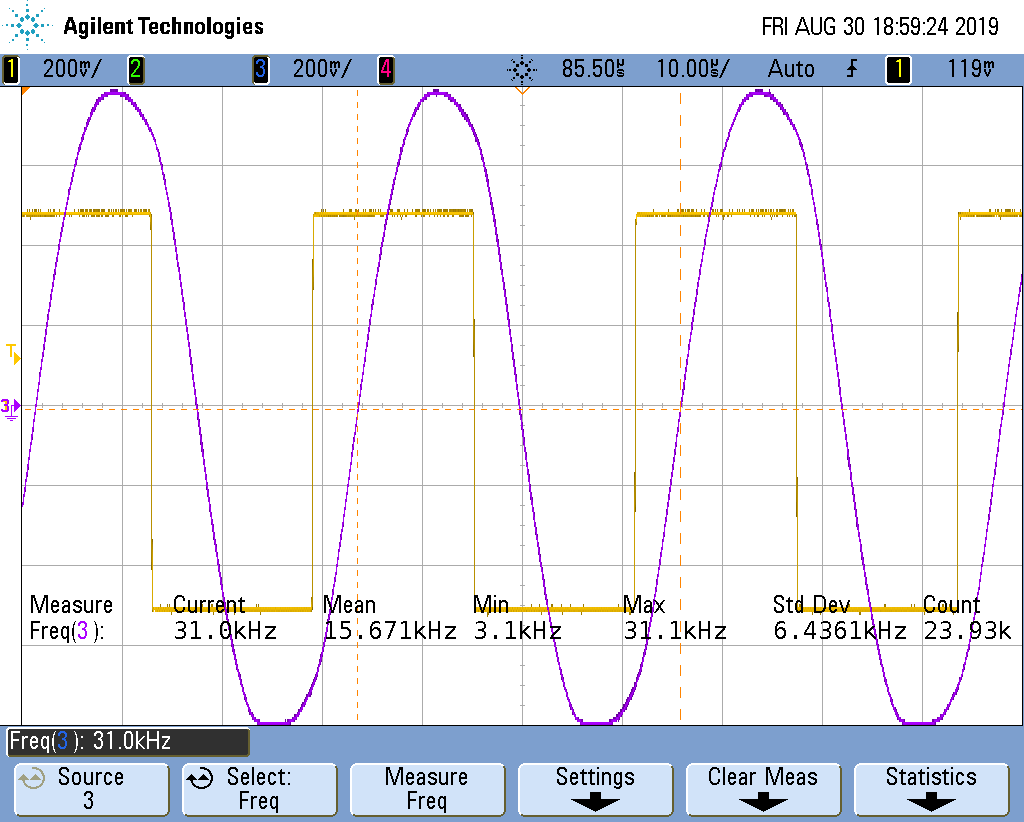
\includegraphics[width=.8\textwidth]{Ejercicio2/Mediciones/A/waveform5.png}  
\end{subfigure}
\begin{subfigure}
  \centering
  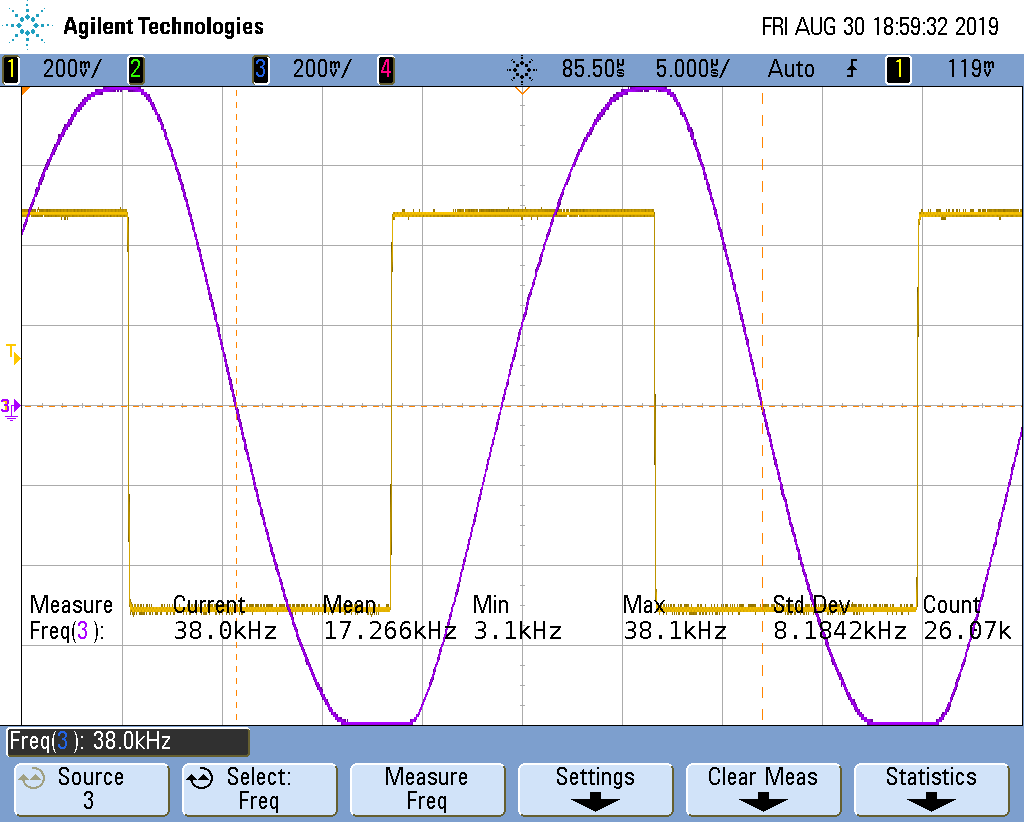
\includegraphics[width=.8\textwidth]{Ejercicio2/Mediciones/A/waveform6.png}  
\end{subfigure}
\end{figure}

\begin{figure}[H]
\centering
\begin{subfigure}
  \centering
  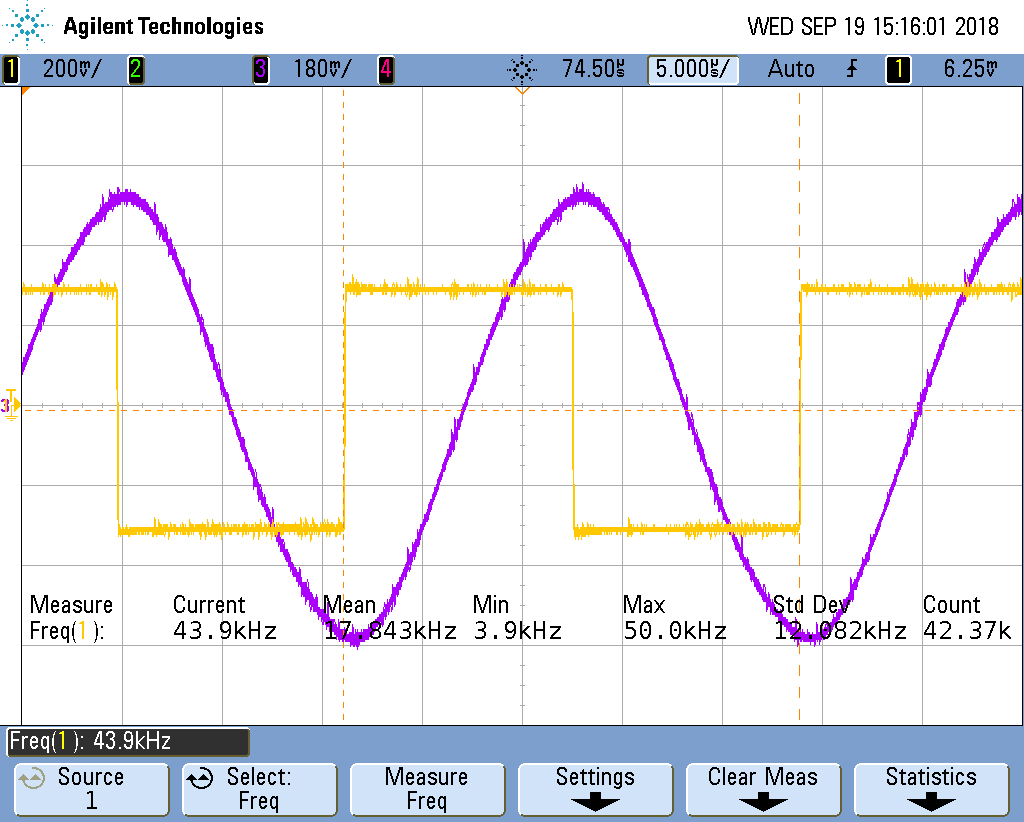
\includegraphics[width=.8\textwidth]{Ejercicio2/Mediciones/A/waveform7.png}  
\end{subfigure}
\begin{subfigure}
  \centering
  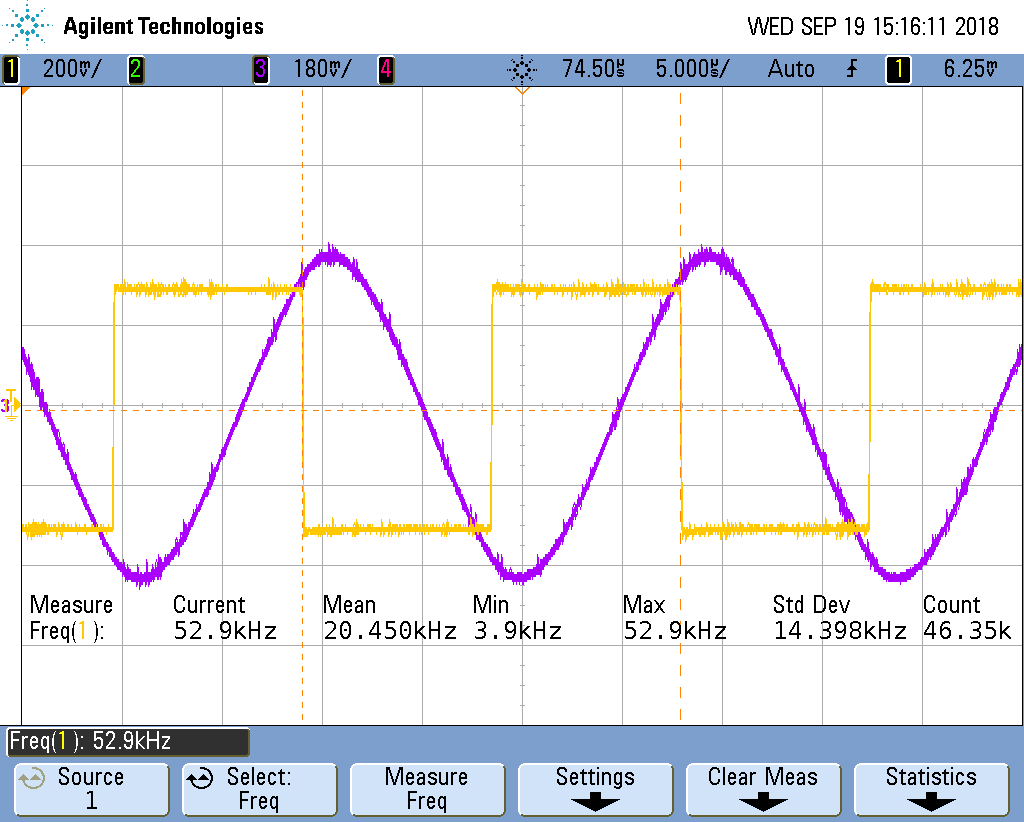
\includegraphics[width=.8\textwidth]{Ejercicio2/Mediciones/A/waveform8.png}  
\end{subfigure}
\begin{subfigure}
  \centering
  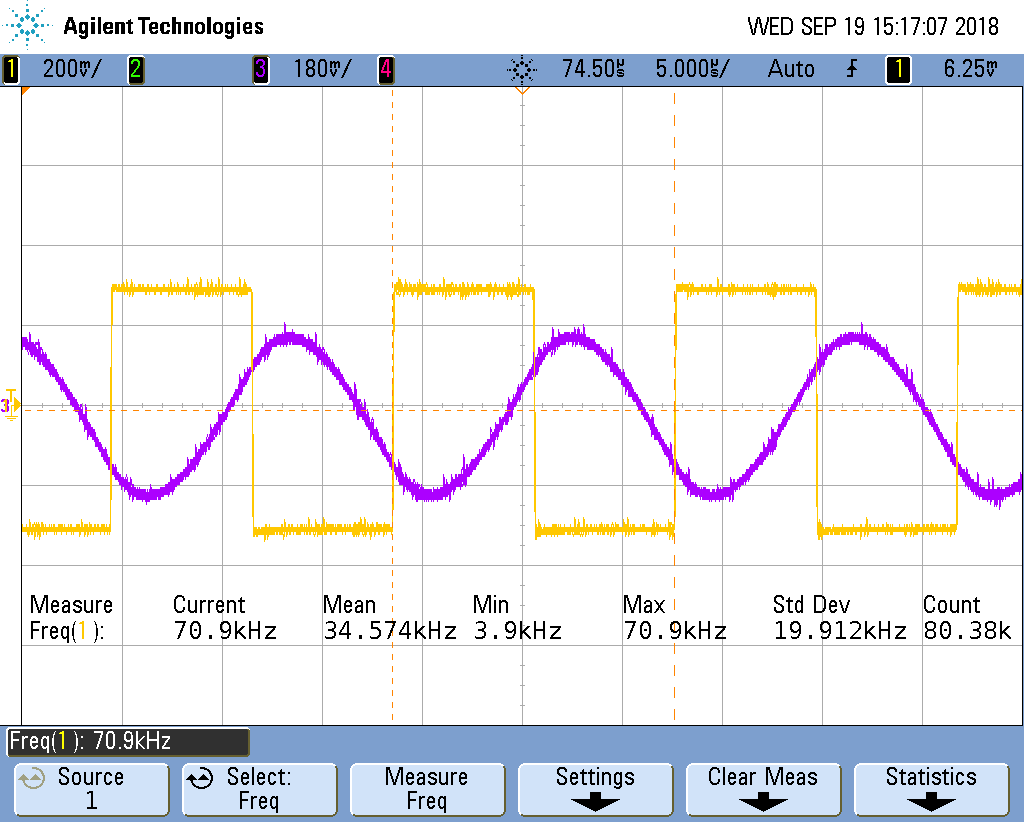
\includegraphics[width=.8\textwidth]{Ejercicio2/Mediciones/A/waveform9.png}  
\end{subfigure}
\caption{Formas de onda frente a un barrido de frecuencia.}
\label{fig:fig}
\end{figure}

A bajas frecuencias, se contempla como si bien la salida del circuito tiene un pequeño tiempo de establecimiento, esta termina copiando a la señal de entrada. En cuanto se sube la frecuencia, la salida del circuito no logra establecerse por completo en lo que dura la cuadrada. Esto genera que la salida del circuito se vea cada vez más como una sinusoidal en cuanto se sube la frecuencia de entrada.

Luego de realizar el análisis de la forma de onda anterior, se obtuvo el diagrama de BODE del sistema. Es así que se compara este con el teórico y con el simulado.

\begin{figure}[H]
	\centering
	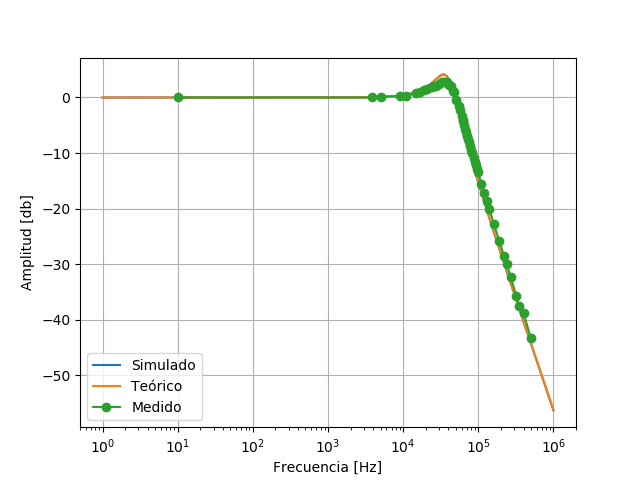
\includegraphics[width=0.9\textwidth]{Ejercicio2/Mediciones/Modulo.png}
\caption{Comparación de diagramas de Bode en módulo.}
	\label{fig:bodemod}
\end{figure}
\begin{figure}[H]
	\centering
	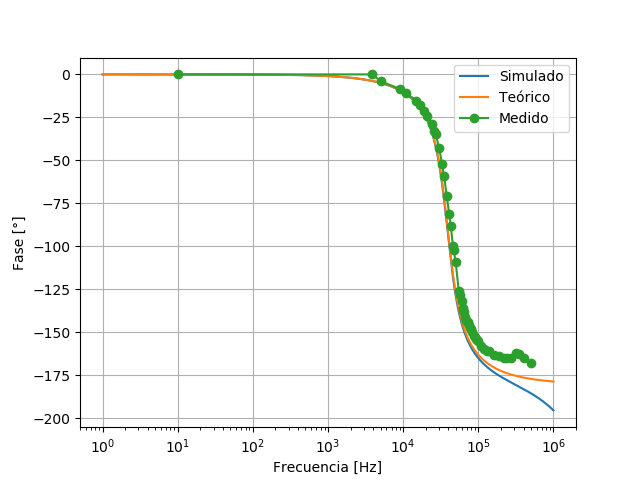
\includegraphics[width=0.9\textwidth]{Ejercicio2/Mediciones/Fase.png}
\caption{Comparación de diagramas de Bode en fase.}
	\label{fig:bodefase}
\end{figure}
%%%%%%%%%%%%%%%%%%%%%%%%%%%%%%%%%%%%%%%%%%%

\subsection{Caso R nula}
\subsubsection{Consideraciones teóricas}
Se analizó el circuito de la figura \ref{fig:rlc} con $R=0\Omega$, i.e. un circuito LC. Teóricamente, el circuito debería oscilar armónicamente, ya que no hay pérdida de energía. Por supuesto, esto no ocurre ya que tanto el cable como el inductor y el capacitor tienen resistencias internas, por lo que sí habrá disipación de energía y las oscilaciones decaerán en cada ciclo.
Los valores teóricos son
\begin{itemize}
  \item frecuencia de oscilación ($f_t$)$=\frac{1}{2\pi}\frac{1}{\sqrt{LC}}\approx 39 kHz$
  \item tiempo de establecimiento ($t_s)$ $\rightarrow \infty$
  \item valor de sobrepico ($M_p$)$=1 V$
\end{itemize}
\subsubsection{Mediciones}

Al realizar la medición se pudo comprobar como el circuito no se comporta como un LC ideal, actuando como un subamortiguado con un factor de calidad muy grande. Se logró medir la pseudofrecuencia de oscilación, siendo esta $f_t= 41,3 kHz$, el tiempo de establecimiento de $5\%$ de $275\mu s$ y finalmente la magnitud del sobrepico, siendo esta $M_p=1,3 V$.

%%%%%%%%%%%%%%%%%%%%%%%%%%%%%%%%%%%%%%%%%%%

\subsection{Caso R tal que $M_p=0,15V_i$}
\subsubsection{Consideraciones teóricas}
Para este caso, excitando al circuito con una señal cuadrada de $5 V_{pp}$, se busca R tal que el valor máximo de sobrepico $M_p=0,15V_i=0,75$
Para hallar R, del desarrollo anterior se tiene que $M_p=0,75\Rightarrow \xi=0,51=R\sqrt{\frac{C}{L}}\frac{1}{2} \Rightarrow R=125,55\Omega $
Luego, los valores teóricos son (utilizando las mismas fórmulas presentadas en la sección del pasabajos) 
\begin{equation}
    f_t=\frac{1}{2\pi}w_d=33,7 kHz
\end{equation}

\begin{equation}
    t_s=\frac{ln({\frac{1}{0,05\sqrt{1-\xi^2}}})}{\frac{R}{2L}}=25,3\mu s
\end{equation}
\subsubsection{Mediciones}

\begin{figure}[H]
  \centering
  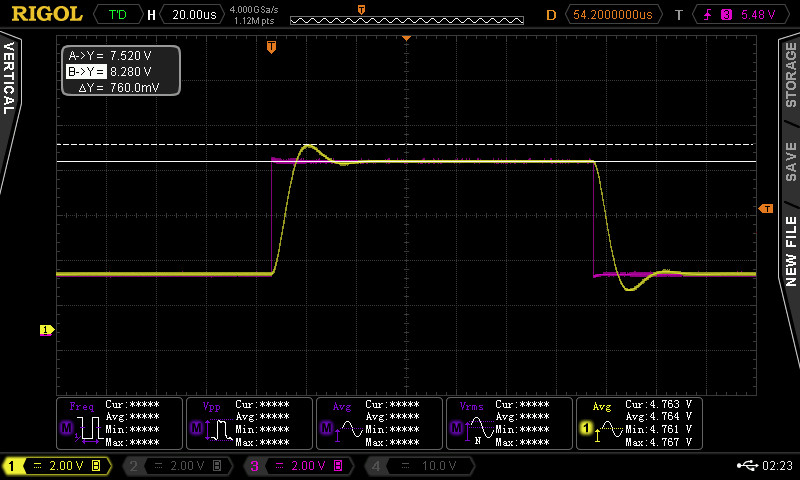
\includegraphics[width=\textwidth]{Mediciones_pendrive_alan/Newfile3.jpeg}  
\end{figure}

Los valores obtenidos de las mediciones fueron:
\begin{itemize}
  \item $f_t= 37,5 kHz$
  \item $t_s=28\mu s$
\end{itemize}
%%%%%%%%%%%%%%%%%%%%%%%%%%%%%%%%%%%%%%%%%%%

\subsection{Caso R tal que el circuito sea críticamente amortiguado}
\subsubsection{Consideraciones teóricas}
Para que el circuito esté críticamente amortiguado se debe verificar \begin{equation}
    \frac{R}{2L}=\frac{1}{\sqrt{LC}}
\end{equation}
Luego \begin{equation}
    R=2\sqrt{\frac{L}{C}}=246,18 \Omega
\end{equation}
En este caso el circuito no oscila, por lo que no hay frecuencia de oscilación del transitorio y $M_p$=0
El tiempo de establecimiento teórico es $t_s=21,4 \mu s$

\subsubsection{Mediciones}

\begin{figure}[H]
  \centering
  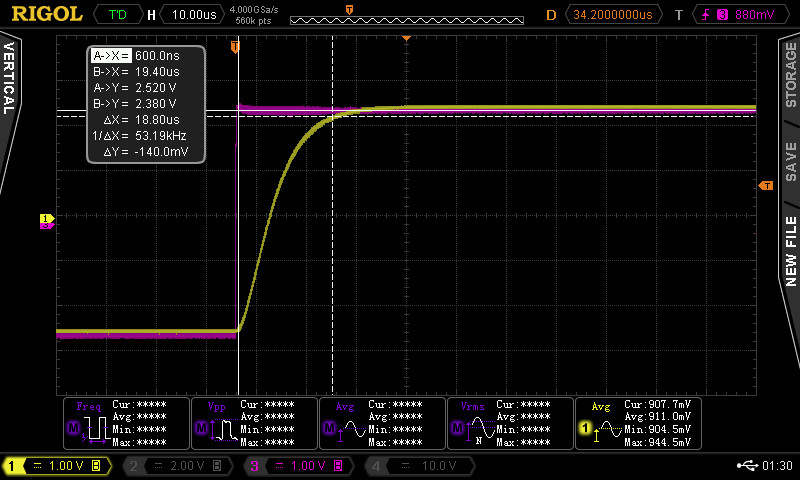
\includegraphics[width=\textwidth]{Mediciones_pendrive_alan/Newfile2.jpeg}  
\end{figure}

Los valores medidos fueron:
\begin{itemize}
  \item $t_s= 18,8 \mu s$
\end{itemize}
%%%%%%%%%%%%%%%%%%%%%%%%%%%%%%%%%%%%%%%%%%%

\subsection{Casos sin buffer}
\subsubsection{$R=0\Omega$}
Teóricamente el circuito debería oscilar armónicamente con una frecuencia $f_t\approx39 kHz$ y $t_s\rightarrow\infty$
Nuevamente el hecho de que todos los elementos poseen resistencias propias causa que las oscilaciones decaigan en cada ciclo. Los valores medidos fueron:
\begin{itemize}
  \item $f_t= 40 kHz kHz$
  \item $t_s=50,4\mu s$
  \item $M_p=1,52 V$
\end{itemize}

\subsubsection{R tal que $M_p=0,15V_i$}
Al quitar el Buffer, la respuesta observada no oscilaba, de donde no hay frecuencia de oscilación del transitorio ni máximo valor de sobrepico. El tiempo de establecimiento del 5\% medido fue $t_s=25\mu s$

%%%%%%%%%%%%%%%%%%%%%%%%%%%%%%%%%%%%%%%%%%%
\section{Filtro pasa banda}
\subsection{Respuesta al escalón}
Se analizó el circuito de la figura \ref{fig:pasabanda}

\begin{figure}[H]
\begin{center}
\begin{circuitikz}
	\node [buffer](buff){};
	\draw (buff.out) to[short] ++(0.25,0) to[L, l = $L$] ++(2,0) to[C, l = $C$] ++(2.5,0) node[](Vcpos){};
	\draw (Vcpos) to[R, l_= $R$, v^= $V_R$] ++(0,-2) node[](Vcneg){};
	\draw (buff.in) to[short] ++(-0.5,0) to[sV, v_=$V_i$] ++(0,-2) to[short] node[ground]{} (Vcneg);
\end{circuitikz}
\caption{Filtro pasabanda}
	\label{fig:pasabanda}
\end{center}
\end{figure}

En este caso la función transferencia es 

\begin{equation}
    H(s)=\frac{sRC}{1+sRC+s^{2}LC}
\label{eq:BandPass}
\end{equation}

La frecuencia de oscilación y el valor de sobre pico teóricos son los mismos que en el caso del filtro pasabajos, calculados en (\ref{equ:fres}) y (\ref{equ:mp}) respectivamente.
Al estar analizando un sistema Lineal Tiempo Invariante (LTI), puede obtenerse la respuesta al escalón como la convolución entre la respuesta impulsiva y la función escalón $u(t)$, que transformando en Laplace, ya que el sistema es causal, permite hallar la respuesta al escalón como \begin{equation}
    Y(s)=H(s)U(s)
\end{equation}
donde $Y(s)$ es la transformada de Laplace de la respuesta al escalón, $U(s)$ es la transformada del escalón y $H(s)$ es la función transferencia del circuito.

Como $U(s)=\frac{1}{s}$ y $H(s)$ está dada por (\ref{eq:BandPass}), antitransformando se obtiene que la respuesta al escalón es 

\begin{equation}
    V_R(t)=\frac{2\sqrt{C}Rsin(\frac{t\sqrt{4L-CR^2}}{2\sqrt{C}L})e^{\frac{-Rt}{2L}}}{\sqrt{4L-CR^2}}
\end{equation}

\subsection{Mediciones}
Se realizaron mediciones de la frecuencia de oscilación del transitorio ($f_t$), del tiempo de establecimiento del 5\% ($t_s$) y del valor de sobrepico ($M_p$)
Los resultados obtenidos fueron:

\begin{itemize}
    \item $f_t=33,7 kHz$
    \item $t_s=40\mu s$
    \item $M_p=400 mV$
\end{itemize}

\subsection{Respuesta en frecuencia}
Se midió la respuesta en frecuencia del circuito (\ref{fig:pasaaltos}) para contrastar que el modelo analítico corresponda con la realidad, además se hizo una simulación en \textbf{LTSpice} obteniendo los siguientes resultados:

\begin{figure}[H]
	\centering
	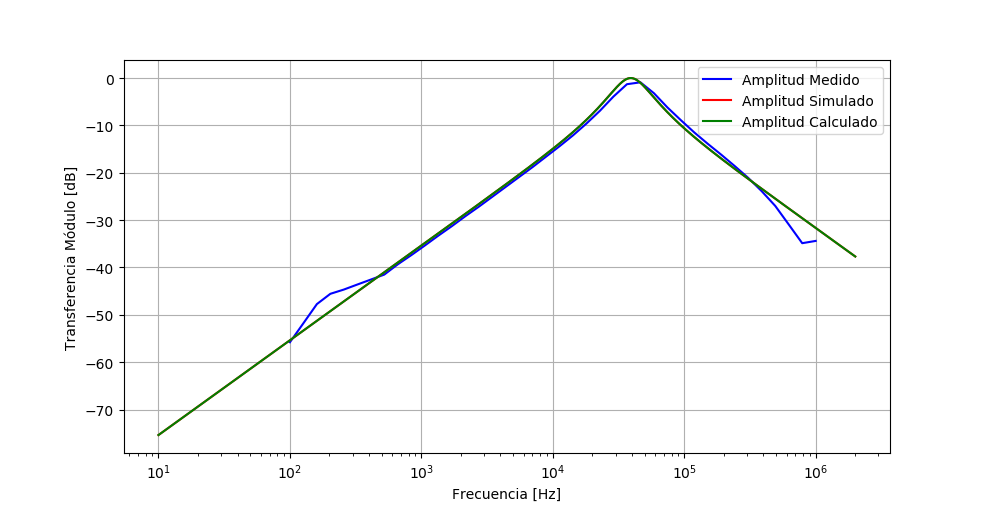
\includegraphics[width=0.9\textwidth]{Bodes_Labo/Fotos/BP.png}
\caption{Comparación de diagramas de Bode en módulo Band-Pass.}
	\label{fig:BODEHP}
\end{figure}

\begin{figure}[H]
	\centering
	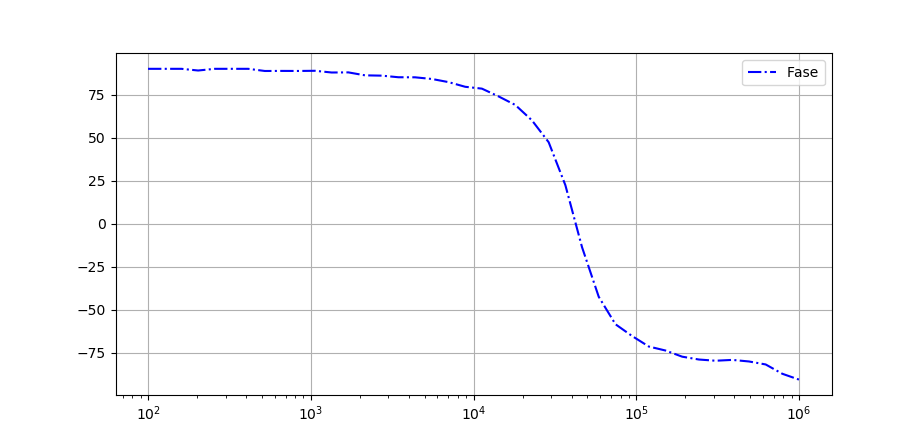
\includegraphics[width=0.9\textwidth]{Bodes_Labo/Fotos/BPP.png}
\caption{Comparación de diagramas de Bode en fase Band-Pass.}
	\label{fig:BODEBPP}
\end{figure}

%%%%%%%%%%%%%%%%%%%%%%%%%%%%%%%%%%%%%%%%%%%
\section{Filtro pasaaltos}
\subsection{Respuesta al escalón}
Se analizó el circuito de la figura \ref{fig:pasaaltos}

\begin{figure}[H]
\begin{center}
\begin{circuitikz}
	\node [buffer](buff){};
	\draw (buff.out) to[short] ++(0.25,0) to[R, l = $R$] ++(2,0) to[C, l = $C$] ++(2.5,0) node[](Vcpos){};
	\draw (Vcpos) to[L, l_= $L$, v^= $V_L$] ++(0,-2) node[](Vcneg){};
	\draw (buff.in) to[short] ++(-0.5,0) to[sV, v_=$V_i$] ++(0,-2) to[short] node[ground]{} (Vcneg);
\end{circuitikz}
\caption{Filtro pasaaltos}
	\label{fig:pasaaltos}
\end{center}
\end{figure}

En este caso la función transferencia es
\begin{equation}
    H(s)=\frac{s^{2}LC}{1+sRC+s^{2}LC}
\label{eq:HighPass}
\end{equation}

Nuevamente, como el denominador de la función transferencia es el mismo que en los casos del filtro pasabanda y pasabajos, los valores teóricos de la frecuencia de oscilación y el sobre pico son los calculados en (\ref{equ:fres}) y (\ref{equ:mp}) respectivamente.
La respuesta al escalón puede calcularse igual que en el caso anterior antitransformando en el dominio de Laplace:
\begin{equation}
    V_L(t)=e^{\frac{-Rt}{2L}}(cosh(\frac{t\sqrt{\frac{CR^2}{4}-L}}{\sqrt{C}L})-\frac{\sqrt{C}Rsinh(\frac{t\sqrt{\frac{CR^2}{4}-L}}{\sqrt{C}L})}{2\sqrt{\frac{CR^2}{4}-L}})
\end{equation}

\subsection{Mediciones}
De la misma manera que el caso anterior, se midió la frecuencia de oscilación del transitorio, el tiempo de estblecimiento del 5\% y el valor de sobrepico. Los resultados obtenidos fueron
\begin{itemize}
    \item $f_t=38,6 kHz$
    \item $M_p=352 mV $
    \item $t_s=49,5 \mu s$
\end{itemize}

\subsection{Respuesta en frecuencia.}
Se midió la respuesta en frecuencia del circuito (\ref{fig:pasaaltos}) para contrastar que el modelo analítico corresponda con la realidad, además se hizo una simulación en \textbf{LTSpice} obteniendo los siguientes resultados:
\begin{figure}[H]
	\centering
	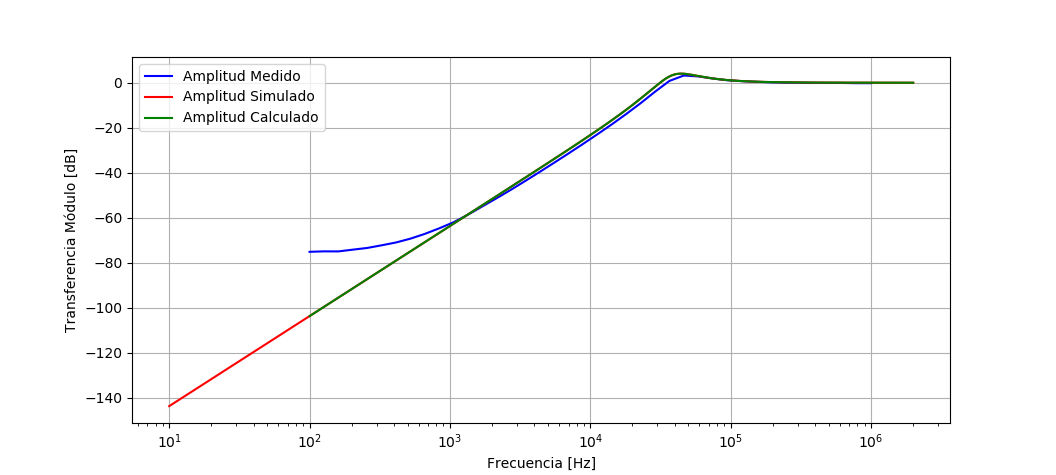
\includegraphics[width=0.9\textwidth]{Bodes_Labo/Fotos/HP.png}
\caption{Comparación de diagramas de Bode en módulo High-Pass.}
	\label{fig:BODEHP}
\end{figure}

\begin{figure}[H]
	\centering
	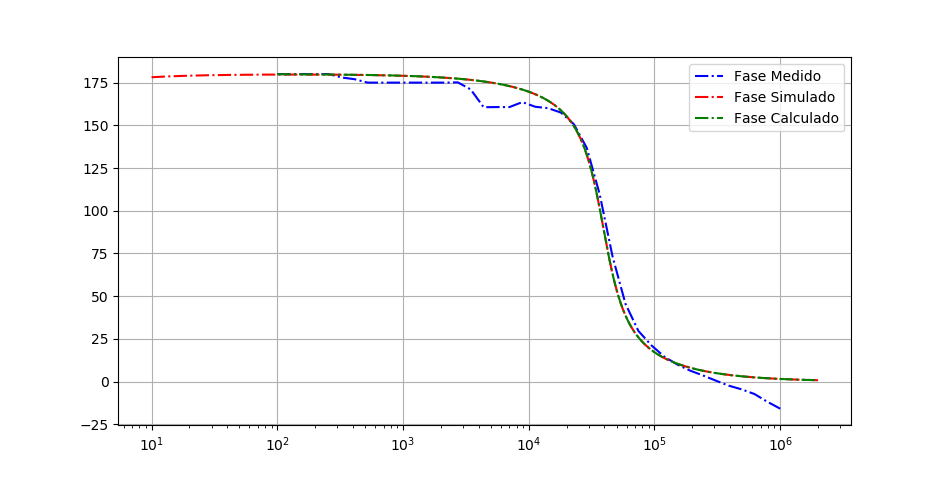
\includegraphics[width=0.9\textwidth]{Bodes_Labo/Fotos/HPP.png}
\caption{Comparación de diagramas de Bode en fase High-Pass.}
	\label{fig:BODEHPP}
\end{figure}
%%%%%%%%%%%%%%%%%%%%%%%%%%%%%%%%%%%%%%%%%%%%%%
\section{Filtro Notch}
\subsection{Respuesta al escalón}
Se analizó el circuito mostrado en la figura \ref{fig:notch}
\begin{figure}[H]
\centering

\begin{circuitikz}
\draw
	(0,0) node[buffer](buff){}
	 (buff.out) to[short] ++(0.25,0)
		 to[R, l = $R$] ++(2,0) 
		 to[L, l = $L$] ++(2.5,0) 
		 node[](Vcpos){}
	(Vcpos) to[C, l_= $C$] ++(0,-2) 
		node[](Vcneg){}
	(buff.in) to[short] ++(-0.5,0) 
		to[sV, v_=$V_i$] ++(0,-2) 
		 node[ground]{} (Vcneg)
	(3.5,0) to [open,v=$V_o$] (3.5,-2)
;
\end{circuitikz}
\caption{Filtro Notch}
	\label{fig:notch}
\end{figure}

En este caso la transferencia está dada por 

\begin{equation}
    H(s)=\frac{1+s^ {2}LC}{1+sRC+s^ {2}LC}
\label{eq:BandReject}
\end{equation}

Los valores teóricos de la frecuencia de oscilación y el sobre pico son, nuevamente, los de (\ref{equ:fres}) y (\ref{equ:mp})

De forma similar a los 2 casos anteriores, antitransformando Laplace se puede obtener la respuesta al escalón en el dominio del tiempo
\begin{equation}
    V_o(t)=1-\frac{2\sqrt{C}Rsin(\frac{t\sqrt{4L-CR^2}}{2\sqrt{C}L})e^{\frac{-Rt}{2L}}}{\sqrt{4L-CR^2}}
\end{equation}

A continuación se presenta la respuesta observada en el osciloscopio.
\begin{figure}[H]
	\centering
	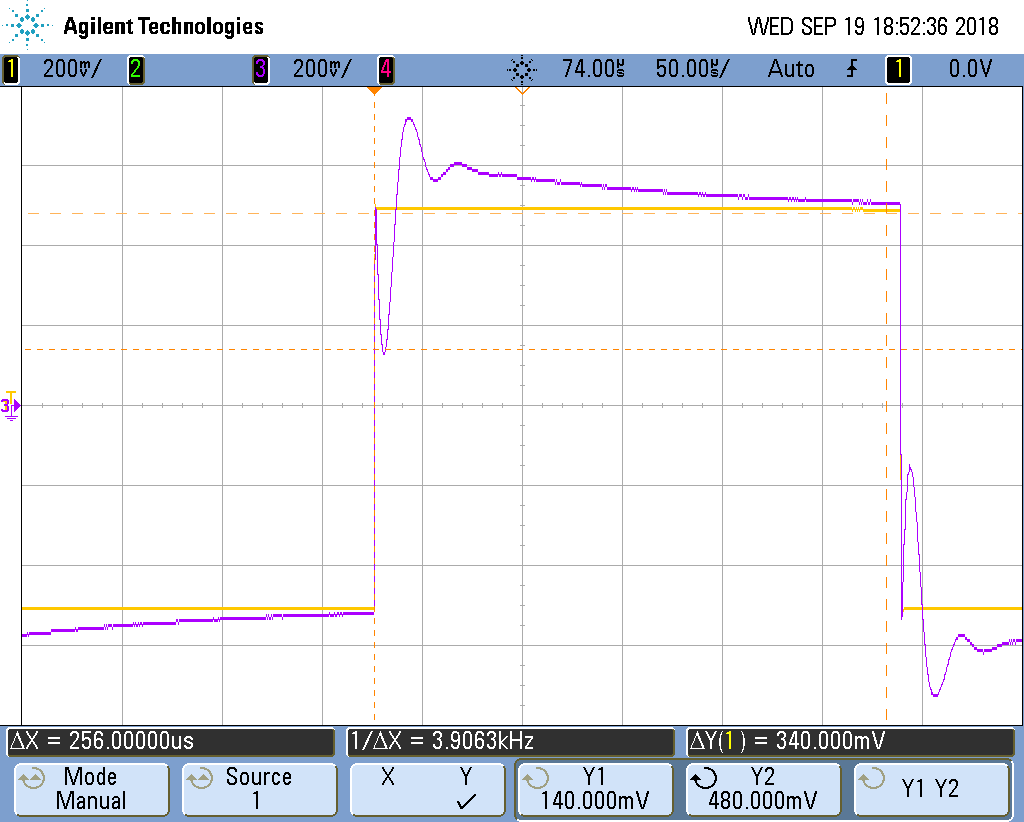
\includegraphics[width=0.9\textwidth]{Mediciones_pendrive_alan/ej4sobrepiconotch.png}
\caption{Respuesta al escalón del circuito en configuración Notch}
	\label{fig:notchescalon}
\end{figure}


\subsection{Mediciones}
Se midió la frecuencia de oscilación del transitorio, el valor de sobrepico y el tiempo de establecimiento del 5\%, obteniéndose
\begin{itemize}
    \item $f_t=38,3 kHz$
    \item $M_p=395 mV$
    \item $t_s=23 \mu s$
\end{itemize}

\subsection{Respuesta en frecuencia}
Se midió la respuesta en frecuencia del circuito (\ref{fig:pasaaltos}) para contrastar que el modelo analítico corresponda con la realidad, además se hizo una simulación en \textbf{LTSpice} obteniendo los siguientes resultados:
\begin{figure}[H]
	\centering
	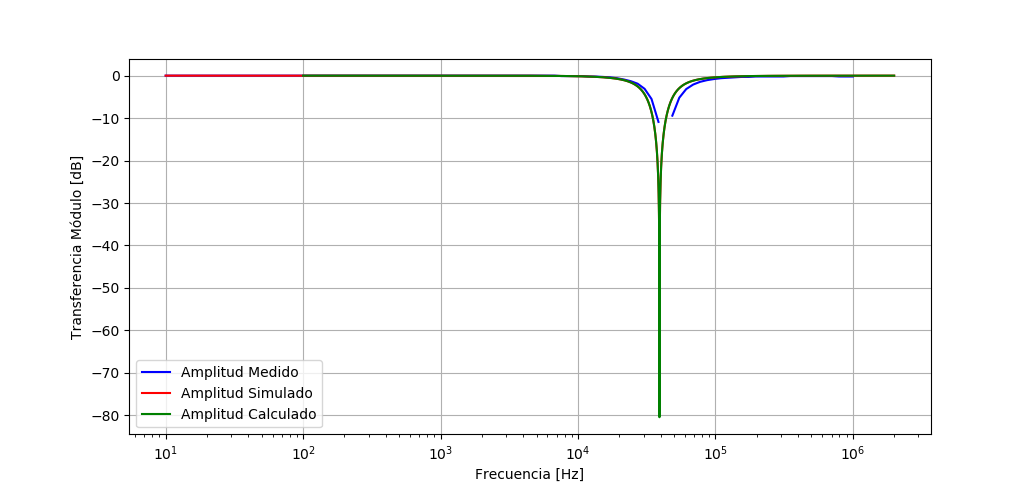
\includegraphics[width=0.9\textwidth]{Bodes_Labo/Fotos/BR.png}
\caption{Comparación de diagramas de Bode en módulo Notch.}
	\label{fig:BODEBR}
\end{figure}

\begin{figure}[H]
	\centering
	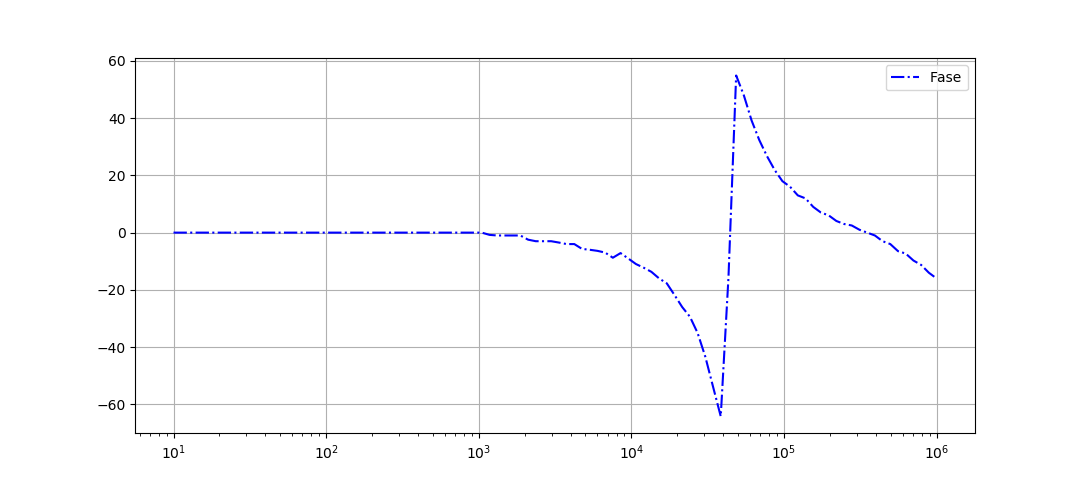
\includegraphics[width=0.9\textwidth]{Bodes_Labo/Fotos/BRP.png}
\caption{Comparación de diagramas de Bode en fase Notch.}
	\label{fig:BODEBRP}
\end{figure}
%%%%%%%%%%%%%%%%%%%%%%%%%%%%%%%%%%%%%%%%%%%%
\section{Medición del factor de calidad}
\subsection{Q Teórico}
Se calculó el valor del factor de calidad de forma teórica según 

\begin{equation}
    Q=\frac{1}{2\xi}=1,51
\end{equation}

Luego, para cada una de las configuraciones anteriores (pasabajos, pasaaltos, pasabanda y notch) se midió el factor de calidad y se lo comparó con el teórico.
\subsection{Q High/Low/Band-Pass}
Para medir el Q del circuito se puede apreciar que si en las ecuaciones (\ref{eq:HighPass}) , (\ref{eq:BandReject}) , (\ref{equ:hrlc}) se evalúa la función en $\omega_0 \implies |H(j\omega_0)|=Q$. El error de obtener el Q del circuito se reduce a errores humanos y de instrumental a la hora de la medición.

\subsection{Q Notch}
En este caso no era tan simple como evaluar la transferencia en un valor dado a que si se evalúa $H(j\omega_0)=0$, se optó por medir la respuesta al escalón, y de allí obtener el sobre pico, el cual esta ligado al $\xi$ por la siguiente ecuación:
\begin{align}M_p = e^{\frac{\pi \cdot \xi}{\sqrt{1-\xi^2}}} \end{align}

\begin{equation}
Q =  \frac{1}{2} \frac{\sqrt{ln(M_p)^2 + \pi^2}}{ln(M_p)}
\end{equation}

obteniendo la siguiente medición:
\begin{figure}[H]
	\centering
	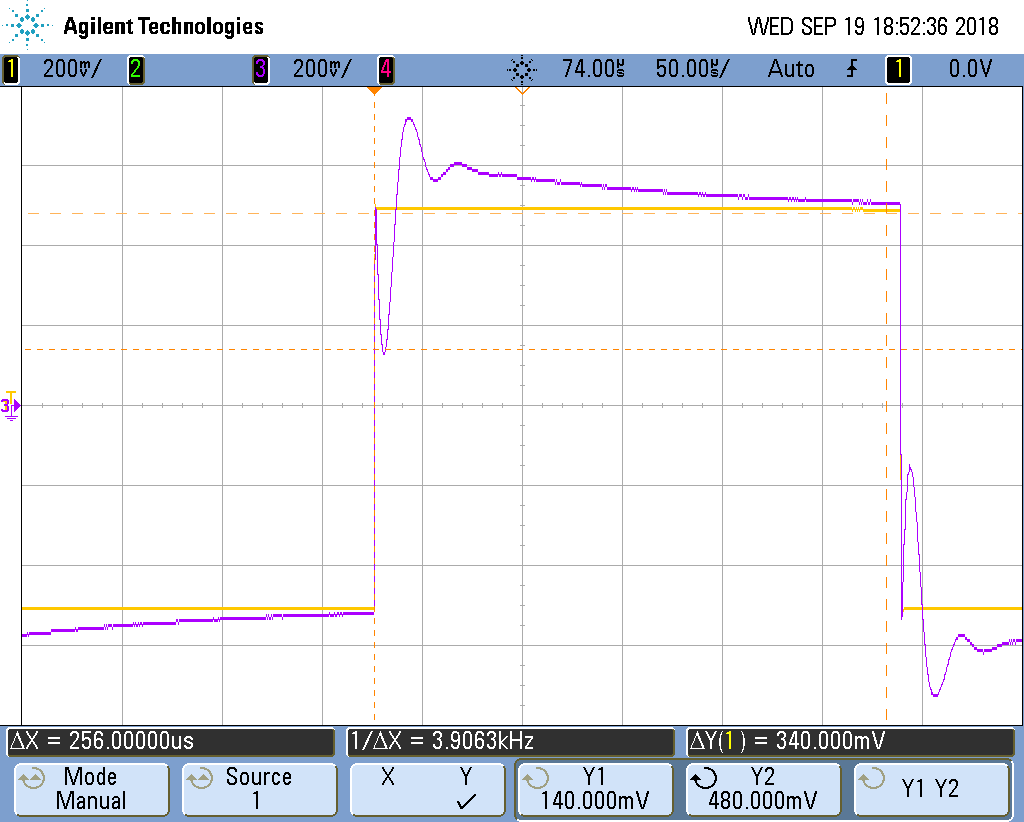
\includegraphics[width=0.9\textwidth]{Mediciones_pendrive_alan/ej4sobrepiconotch.png}
\caption{Sobre pico de la respuesta al escalón en el Notch.}
	\label{fig:Overshoot5}
\end{figure}

y un valor de Q de $1,539$.

\end{document}
